\section{System and Data}
\label{sec:data-collection}

In this section, we describe our system -- Android platform and Pebble platform. We then briefly cover the experiement setup. \ben{maybe this should be in introduction.} Throughout the paper, we use {\em Phone} for mobile phones, and {\em Glass}, {\em Pebble} for Google Glass and Pebble Smartwatch, respetively.


\subsection{Android Platform}
\label{sec:android-platform}

Our Android application is adapted from BearLoc\footnote{BearLoc is developed by Software Defined Buildings (SDB) group at Berkeley; the intial goal of that project is to provide an open-source implementation that is targeted at indoor semantic localization service.}. We built a continous sensor monitoring application on top of \texttt{BearLocService} which makes sensor data collection

Our initial application involves sampling all sorts of sensor data from Android platform, including acclerometer, gyroscope, magnetic field, light, GPS, WiFi signals, etc. However, through some preliminary study, we have found that mobile phones and Google Glass cannot easily handle the extensive sensing tasks, especially when we are trying to sample acceleration in a relative high frequency. Since we are interested in the comparison among these wearable devices and Pebble only has a 3D accelerometer, we implemented our Android application only for sampling acclerometer data.

The sensor data is obtained through \texttt{onSensorChanged()} API provided by Android OS. The sampling frequency is resource adaptive -- it turns out to be 100Hz for phones and 50Hz for Glass. 

Once the data is measured, we record the time in millisecond accuracy by calling \texttt{System.currentTimeMillis()}. To extract the data, we logged the data locally by writing to a \texttt{csv} file and also post a HTTP request that saves the data to \texttt{MongoDB}.

\subsection{Pebble Platform}
\label{sec:pebble-platform}

The Pebble accelerometer data collection application is based on \texttt{AccelerometerService} API provided by Pebble OS. We register a callback function as the handler whenever accelerometer data is available. The callback function operates on \texttt{AccelData} which already has a field of timestamp in millisecond accuracy. 

The data storage and transmission is supported by \texttt{DataLogging} API which requires a customized Android application that uses Pebble SDK to retrieve logs by application universally unique identifier (UUID). We have also developed this accompany Android application for retrieving the data and writing them into a \texttt{csv} file for data analysis.

\subsection{Accelerometer Data}
\label{sec:accelerometer-axes}

On both Android and Pebble platform, the acclerometer coordinate system is defined relative to the device's screen (see Figure~\ref{fig:coordinate}). When the user is facing the screen, the axes are:
\begin{itemize}
\item x: horizontal and points to the right.
\item y: vertical and points up.
\item z: points towards the outside of of the screen face.
\end{itemize}

 
%% 04-20 17:40:46.392    4187-4187/name.benzhang.hellostep.app I/HelloStep﹕ {Sensor name="MPL Accelerometer", vendor="Invensense", version=1, type=1, maxRange=19.6133, resolution=0.039226603, power=0.0, minDelay=1000}

%% { "_id" : ObjectId("536f303fe0323929bee2cf88"), "vendor" : "STMicroelectronics", "power" : 0.23000000417232513, "min delay" : 20000, "resolution" : 0.01362034771591425, "sysnano" : NumberLong("170075408653778"), "epoch" : NumberLong("1399795756898"), "version" : 1, "max range" : 19.613300323486328, "type" : "sensor info", "model" : "KR3DM 3-axis Accelerometer", "sensor" : "accelerometer", "id" : "9026086e-bd07-3f96-9622-757da2907a93" }

However, the data differs in range, resolution and sample frequency. We use $g$ to denote the gravitational accelerometer constant (normal $9.81 m/s^2$). In Table~\ref{tab:sensorinfo}, we have listed the sensor information. Note that in our project, we have been using Samsung Galaxy S II, so the information is for that particular device. 

\begin{table}
  \centering
  \begin{tabular}{c|c|c|c}
    \hline
    Device & max range & resolution & sample frequency \\
    \hline
    Phone  & 19.6g     & 0.013g     & 100Hz  \\
    Glass  & 19.6g     & 0.039g     & 50Hz   \\
    Pebble & 4g        & 0.008g     & 25Hz   \\
    \hline
  \end{tabular}
  \label{tab:sensorinfo}
  \caption{Sensor information of the devices.}
\end{table}

\begin{figure}
  \centering
  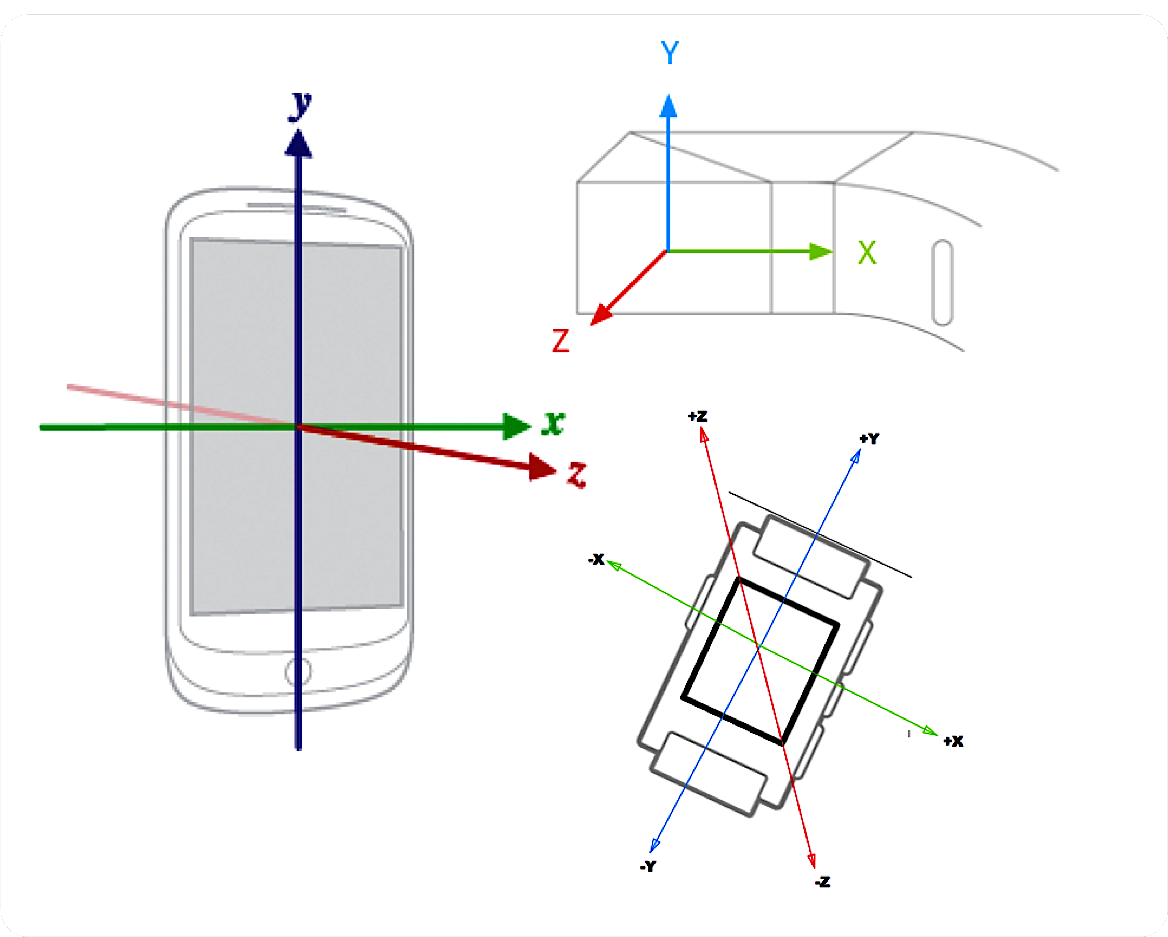
\includegraphics[width=0.9\columnwidth]{figures/coordinates.png}
  \caption{3D co-ordinate system of our hardware platforms.}
  \label{fig:coordinate}
\end{figure}

\subsection{Data Collection}
\label{sec:data-collection-2}

With our data collection platform, we have performed a series of activities and collected the acclerometer data. Figure~\ref{fig:exp} shows how these devices are worn on a user and the experiement is being conducted. To obtain the ground truth, we use an extra iPhone to take videos continuously during the study. The video is manually processed to label the collected acclerometer data.

\begin{figure}
  \centering
  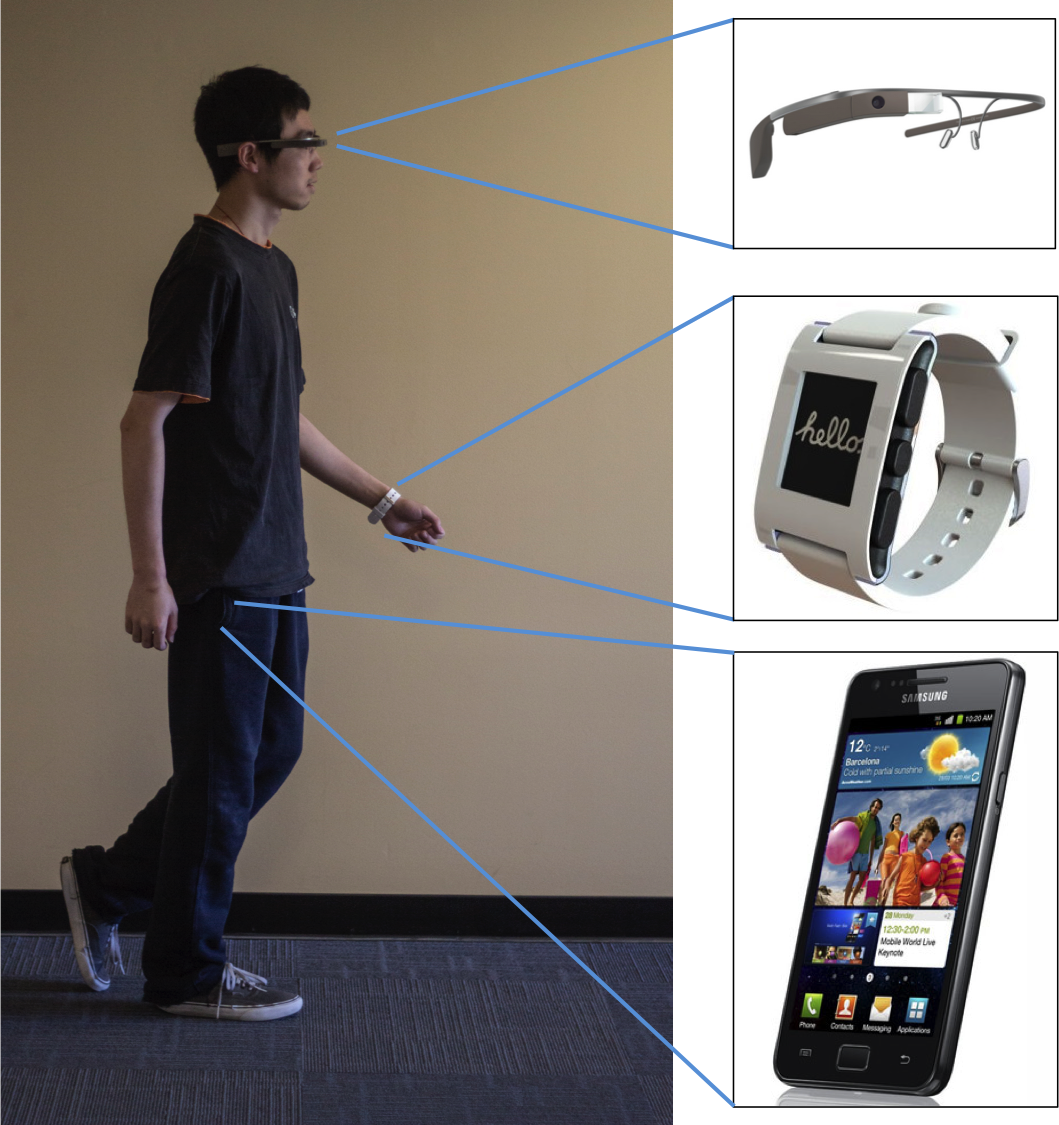
\includegraphics[width=0.9\columnwidth]{figures/experiement_setup.png}
  \caption{Data collection process of simutaneously wearing three different devices and an illustration of their relative positions on the testee's body.}
  \label{fig:exp}
\end{figure}



%%% Local Variables: 
%%% mode: latex
%%% TeX-master: "main"
%%% End: 
